\chapter{Data Layout and Marshaling}
\label{ch:ffi-marshaling}

A structure containing a one-byte tag, a four-byte count, and an eight-byte pointer does not necessarily occupy thirteen bytes.
A byte string containing a zero byte is not necessarily terminated there.
An array with a pointer and shape is not necessarily contiguous.
An adapter must reconcile these distinctions before handing data to native code.
\term{Marshaling} converts values into the representation required at a boundary; it can involve validation, layout, encoding, copying, or constructing views.

\section{Distinguish native layout from a wire format}
\label{sec:ch71-layout}
Assume ordinary unpacked fields with sizes and alignments $(1,1)$, $(4,4)$, and $(8,8)$.
The tag begins at offset $0$.
The count cannot begin at offset $1$; rounding up to alignment $4$ places it at $4$.
The pointer then begins at $8$, and the structure ends at $16$.
Table~\ref{tab:ch71-layout} and Figure~\ref{fig:ch71-padding} work the complete layout.

\begin{table}[htbp]
\caption{Alignment inserts three internal padding bytes in this native layout.}
\label{tab:ch71-layout}
\centering
\begin{tabular}{lrrrr}
\toprule
Field & Size & Alignment & Offset & End \\
\midrule
tag & 1 & 1 & 0 & 1 \\
count & 4 & 4 & 4 & 8 \\
pointer & 8 & 8 & 8 & 16 \\
\bottomrule
\end{tabular}
\end{table}

\begin{figure}[htbp]
\centering
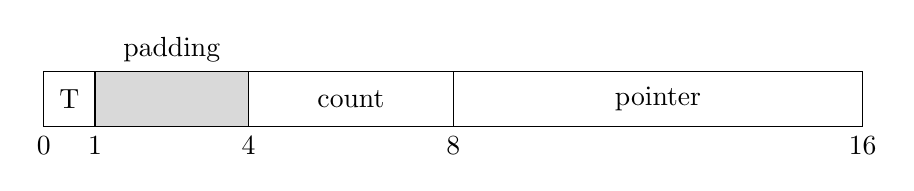
\begin{tikzpicture}[x=0.65cm,y=1cm]
\draw (0,0) rectangle (1,0.7);
\draw[fill=black!15] (1,0) rectangle (4,0.7);
\draw (4,0) rectangle (8,0.7); \draw (8,0) rectangle (16,0.7);
\node at (0.5,0.35) {T}; \node at (6,0.35) {count}; \node at (12,0.35) {pointer};
\foreach \x in {0,1,4,8,16} \node[below] at (\x,0) {\x};
\node[above] at (2.5,0.7) {padding};
\end{tikzpicture}
\caption{Offsets describe native storage, including padding that carries no field value.}
\label{fig:ch71-padding}
\end{figure}

Algorithm~\ref{alg:ch71-layout} computes this simple layout from target-supplied alignments.
For $F$ fields it costs $O(F)$ time and $O(F)$ output storage.
It assumes positive power-of-two alignments, ordinary fields, and representable size arithmetic; a compiler implementation must detect size overflow.
Packing rules, bit-fields, flexible array members, and target-specific aggregate restrictions require additional handling.

\begin{algorithm}[htbp]
\caption{Lay out ordinary fields using supplied target sizes and alignments.}
\label{alg:ch71-layout}
\begin{pseudocode}
\Require fields with sizes $s_i$ and alignments $a_i$; checked arithmetic
\Ensure offsets and total size, or size-overflow diagnostic
\State $p\gets0$; $a\gets1$
\ForAll{fields $i$ in order}
  \State $p\gets\operatorname{roundUp}(p,a_i)$; record offset $p$
  \State $p\gets p+s_i$; $a\gets\max(a,a_i)$
\EndFor
\State return recorded offsets, $\operatorname{roundUp}(p,a)$, and $a$
\end{pseudocode}
\end{algorithm}

Native layout is not a portable serialization format.
Endianness can differ, pointer values belong to an address space, and padding bytes need not have a canonical value~\cite{wg14-2011-c11}.
Comparing an entire structure with a byte comparison can therefore disagree with fieldwise equality.
Likewise, an unaligned packet address must not simply be cast to an arbitrary structure pointer.
Decode explicitly or copy individual scalar representations into suitably aligned objects under a documented representation contract.

\section{Count bytes and validate extents}
\label{sec:ch71-extents}
The companion wire model defines an independent format: one tag byte, four little-endian length bytes, then exactly that many payload bytes.
There is no pointer or native padding in this representation.
For tag $9$ and payload consisting of A, zero, and B, the eight hexadecimal bytes are
\code{09 03 00 00 00 41 00 42}.
The interior zero is data, not a terminator.

Algorithm~\ref{alg:ch71-decode} checks the header before inspecting its length and rejects truncated or trailing data.
The size limit of $1{,}048{,}576$ bytes bounds allocations in the example; it is a resource policy rather than a property of UTF-8 or the ABI.
Decoding a copied payload of $N$ bytes costs $O(N)$ time and storage; validating an already available contiguous packet's extent is $O(1)$.

\begin{algorithm}[htbp]
\caption{Decode a bounded byte record without native-structure casts.}
\label{alg:ch71-decode}
\begin{pseudocode}
\Require packet with known byte extent $N$; payload limit $L$
\Ensure tag and payload, or rejection without an out-of-bounds read
\If{$N<5$} \State reject short header \EndIf
\State read tag byte; decode four-byte little-endian length $n$
\If{$n>L$ or $n\ne N-5$} \State reject inconsistent extent \EndIf
\State return tag and the payload bytes in $[5,N)$
\end{pseudocode}
\end{algorithm}

For native slicing, validate offset $o$ and count $n$ against size $s$ by checking $o\le s$ and then $n\le s-o$.
Checking only $o+n\le s$ can accept wrapped unsigned addition.
Checking a multiplication such as element count times stride similarly requires a division bound before multiplying.
These checks establish arithmetic consistency, not that a caller-supplied raw pointer really designates an allocation of the claimed size.
That remains a native caller obligation.

\section{Strings and arrays carry additional structure}
\label{sec:ch71-strings}
ASCII A followed by U+00E9 has two Unicode code points but three UTF-8 bytes: \code{41 C3 A9}.
A native byte length is three, while a count of code points is two.
Neither count generally measures user-perceived characters.
An interface accepting text must specify encoding, treatment of invalid sequences, normalization requirements if any, and whether interior zeros are allowed.
Our byte-buffer API accepts uninterpreted bytes and makes no text-validity claim.

For arrays, shape and strides matter independently of element type.
A two-row, three-column matrix of 32-bit integers in contiguous row-major storage has byte strides $12$ and $4$.
A view selecting every second column is no longer a contiguous six-element array.
The wrapper can copy into the required order, accept a stride-aware native routine, or reject the view.
It must not silently discard stride information.
Table~\ref{tab:ch71-representations} lists policies that an interface declaration needs to distinguish.

\begin{table}[htbp]
\caption{A pointer alone omits the metadata needed to interpret a value.}
\label{tab:ch71-representations}
\centering
\begin{tabular}{ll}
\toprule
Value & Additional contract \\
\midrule
byte string & byte extent; interior-zero policy \\
text & encoding; validation; length unit \\
array view & element format; shape; strides; access mode \\
native structure & target layout; alignment; field interpretation \\
serialized record & byte order; version; explicit offsets or lengths \\
\bottomrule
\end{tabular}
\end{table}

The CPython wrapper requests a contiguous byte buffer through the documented buffer interface and releases the export after copying~\cite{python-2026-capi}.
Its test rejects a strided memory view rather than misreading it.
The Lua wrapper uses the explicit string length, so a string containing zero and byte $255$ survives unchanged.
Neither adapter routes binary data through a zero-terminated-string conversion.

\section{Zero-copy is a lifetime and mutation protocol}
\label{sec:ch71-zero-copy}
\term{Zero-copy interoperability} shares an existing data region rather than copying its payload across the boundary.
It still requires metadata, owner retention, valid alignment, and a rule preventing invalidating resize or relocation during use.
Read-only access through one wrapper does not freeze the underlying region against other aliases.
Concurrent mutation needs synchronization or a snapshot contract.

Figure~\ref{fig:ch71-copy} contrasts a copy with a shared view.
In the copy path, later changes to the source do not affect the native object.
In the view path, releasing the source owner before the consumer completes invalidates the view even if the pointer bits remain unchanged.
For small payloads a copy can simplify ownership enough to outweigh its cost; that tradeoff needs measurement on the actual workload.

\begin{figure}[htbp]
\centering
\begin{tikzpicture}[node distance=12mm and 14mm]
\node[basic block] (source) {source allocation};
\node[basic block,below left=of source] (copy) {independent native copy};
\node[basic block,below right=of source] (view) {view retains source owner};
\draw[cfg edge] (source)--node[left,font=\small]{copy bytes}(copy);
\draw[cfg edge] (view)--node[right,font=\small]{keep alive}(source);
\end{tikzpicture}
\caption{Copying separates mutation and lifetime; a view preserves a dependency on the source.}
\label{fig:ch71-copy}
\end{figure}

The case study chooses copies on both entry and return.
Its test mutates and resizes a Python bytearray after construction and verifies the native snapshot still contains the original four bytes.
A production zero-copy variant would need a wrapper object retaining the export until close, a policy for outstanding views at close, and a corresponding native access discipline.
Adding only a pointer field would not implement that variant.

\section{Exercises}
\label{sec:ch71-exercises}
\begin{enumerate}
\item\label{ex:ch71-layout} Compute offsets and size for the same fields reordered as pointer, tag, count.
Does reordering reduce the total under the stated alignments?
\item\label{ex:ch71-packet} Encode tag $9$ and the three-byte payload A, zero, B.
Explain why removing the last byte and appending an extra byte are both rejected.
\item\label{ex:ch71-overflow} Consider a four-byte buffer.
Evaluate the safe extent checks for $(o,n)=(4,0)$ and for $(o,n)=(1,\mathrm{SIZE\_MAX})$.
\item\label{ex:ch71-view} A two-by-three int32 matrix has row stride $12$ and column stride $4$.
Give the offsets of the view selecting columns zero and two, and explain why treating it as four contiguous int32 values is wrong.
\end{enumerate}

\section{Further reading}
\label{sec:ch71-reading}
C11 describes structure padding, alignment, and object representations~\cite{wg14-2011-c11}.
The Python buffer documentation specifies shape, stride, format, and export-release obligations~\cite{python-2026-capi}.
Lua's explicit-length string API provides a compact example of binary-safe marshaling~\cite{ierusalimschy-2026-lua}.
